\documentclass{article}
\usepackage[utf8]{inputenc}
\usepackage{graphicx}

\title{Camera based Water Stage and Discharge Prediction with Machine Learning}
\author{
Ernesto Adrián Álvarez Salazar  A00227490\\
Carlos Javier Leal Beltrán  A01741355\\
Carlos Moisés Chávez Jiménez  A01637322\\
Luis Armando Salazar López  A01114901\\
}
\date{Septiembre 2022 - Diciembre 2022}

\usepackage{listings}
\usepackage{color}

\definecolor{dkgreen}{rgb}{0,0.6,0}
\definecolor{gray}{rgb}{0.5,0.5,0.5}
\definecolor{mauve}{rgb}{0.58,0,0.82}

\lstset{frame=tb,
  language=Python,
  aboveskip=3mm,
  belowskip=3mm,
  showstringspaces=false,
  columns=flexible,
  basicstyle={\small\ttfamily},
  numbers=none,
  numberstyle=\tiny\color{gray},
  keywordstyle=\color{blue},
  commentstyle=\color{dkgreen},
  stringstyle=\color{mauve},
  breaklines=true,
  breakatwhitespace=true,
  tabsize=3
}

\begin{document}

\maketitle

\section{Introducción}

La medición y el modelado precisos del nivel y la descarga de la corriente son importantes para la gestión diaria del agua, el pronóstico y la gestión de inundaciones, la evaluación del cumplimiento de los acuerdos de uso del agua y el diseño de embalses, sistemas de suministro de agua, puentes y alcantarillas (Boiten, 2008). Los datos continuos de series de tiempo de medidores de flujo también son críticos para calibrar y/o validar modelos de aguas superficiales y subterráneas, mientras que las brechas en estos datos aumentan la incertidumbre en las predicciones de un modelo.  El nivel de la corriente normalmente se mide con sensores flotantes, de presión, ópticos y acústicos (Turnipseed y Sauer, 2010).  Estos sensores tradicionales pueden fallar y requerir un mantenimiento regular, los cuales son costosos.  Como resultado, es posible que se produzcan lagunas en los registros de flujo y descarga debido a una instalación incorrecta (p. ej., especialmente durante estudios a corto plazo, cuando las características del sitio no son bien conocidas), fallas en los equipos y/o brechas en el financiamiento de los programas de monitoreo.  Por supuesto, las cámaras también pueden fallar, pero pueden proporcionar una redundancia económica con información que no está disponible en los sensores que emiten mediciones escalares individuales.  Por ejemplo, las imágenes proporcionan una verificación visual de las condiciones hidrológicas, incluida la presencia de hielo, obstrucciones o cambios importantes en la geometría del canal.  En este estudio, nos enfocamos en un enfoque de monitoreo pasivo que utiliza imágenes de lapso de tiempo que se pueden combinar con mediciones de sensores tradicionales que son adecuadas para llenar los vacíos en los registros de caudales.



\section{Tratamiento Inicial de los Datos}

Para comenzar a trabajar con los datos, es necesario que pasen por un proceso de preparación que nos permita obtener la mejor parte de ellos. Este proceso se divide en tres etapas: Limpieza, Transformación y Visualización. A continuación desglosaremos las fases involucradas a este proceso:

    \subsection{Limpieza de los datos}

        La limpieza es la primera y una etapa fundamental del tratamiento de la información. Aquí se busca eliminar la mayor cantidad de imperfecciones que pudieramos llegar a encontrar. Cosas como valores faltantes, datos fuera de rango, dividir la información disponible en "entrenamiento" y "pruebas", eliminar columnas innecesarias para el análisis, etc.\\

        \begin{center}
        \begin{tabular}{ |c|c|c|} 
        \hline
        SensorTime & CaptureTime & Filename\\ 
        Agency & SiteNumber & TimeZone\\ 
        Stage  & Discharge & CalcTimestamp\\ 
        width & height & exposure \\ 
        fNumber & isoSpeed  & shutterSpeed    \\ 
        grayMean & graySigma & entropyMean   \\ 
        entropySigma & hMean & hSigma  \\ 
        sMean & sSigma & vMean  \\ 
        vSigma & areaFeatCount & grayMean 0 \\  
        graySigma 0  & entropyMean 0  & entropySigma 0 \\ 
        hMean 0      & hSigma 0     & sMean 0       \\ 
        sSigma 0     & vMean 0      & vSigma 0 \\ 
        grayMean 1   & graySigma 1  & entropyMean 1        \\ 
        entropySigma 1      & hMean 1      & hSigma 1      \\ 
        sMean 1      & sSigma 1     & vMean 1       \\ 
        vSigma 1     & WeirAngle    & WeirPt1X        \\ 
        WeirPt1Y       & WeirPt2X       & WeirPt2Y        \\ 
        WwRawLineMin   & WwRawLineMax   & WwRawLineMean \\ 
        WwRawLineSigma & WwCurveLineMin & WwCurveLineMax  \\ 
        WwCurveLineMean     & WwCurveLineSigma &      \\ 
        \hline
        \end{tabular}
        \end{center}

       \begin{center}
           \textbf{Clases disponibles en nuestro archivo de datos.} \\
       \end{center}     
        

    \subsection{Transformación de los datos}
        Una vez revisados los datos, entendemos que debemos transformarlos para generar gráficos y diagramas que faciliten la búsqueda de patrones y la determinación de si será necesario un modelo predictor de regresión o de clasificación.
        
        Para esto, revisamos el dataframe con la información proporcionada. Encontramos que primero debemos ordenar los datos con base en el timestamp. Esta variables que indican el tiempo con el que fueron realizadas las capturas de datos. Dentro del dataframe se proporcionan tres variables para indicar el tiempo de captura: "CaptureTime","SensorTime" y "CalcTimestamp", y cada una de estas contiene un formato distinto y a primera instancia nada fácil de trabajar, lo que indica que tenemos que separarlas para que queden enumeradas de una en una. Desarrollamos un método para tratar las fechas consiguiendo así, un orden en el formato de la captura de datos. En cuanto a lo demás, los datos venían en buenas condiciones, por lo que no tuvimos que arreglar valores nulos. \\

    \subsection{Visualización de los datos}\\

        Siendo las variables "Stage" y "Discharge" las que nos iteresan predecir con un modelo, las comparamos con el resto de las variables para ir descartando las de menor correlacion.

        \begin{center}
            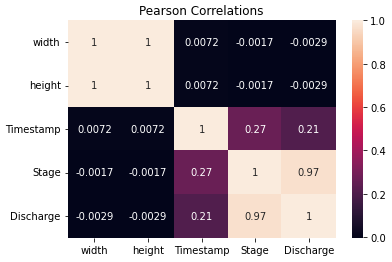
\includegraphics{images/Corr_pearson1.PNG} 
            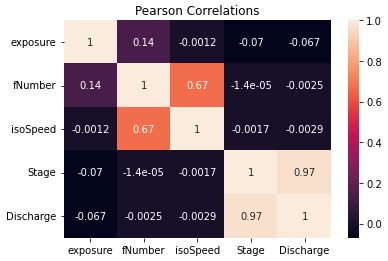
\includegraphics{images/Corr_pearson2.PNG} 
            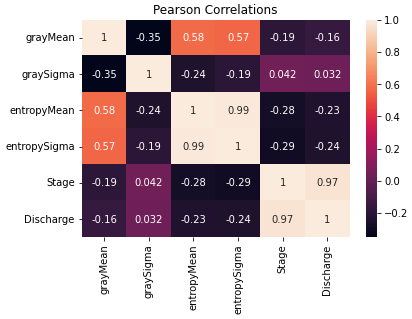
\includegraphics{images/Corr_pearson3.PNG} 
            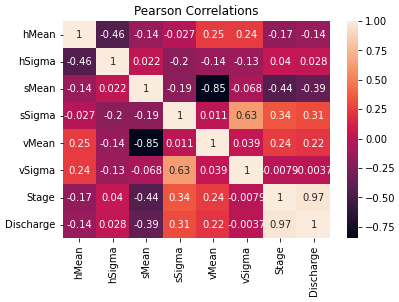
\includegraphics{images/Corr_pearson4.PNG} 
            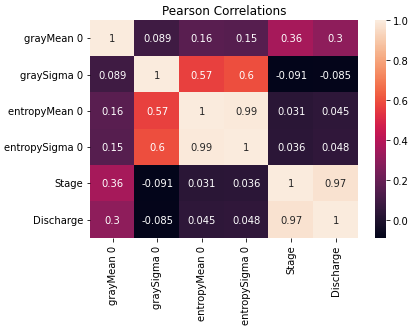
\includegraphics{images/Corr_pearson5.PNG} 
            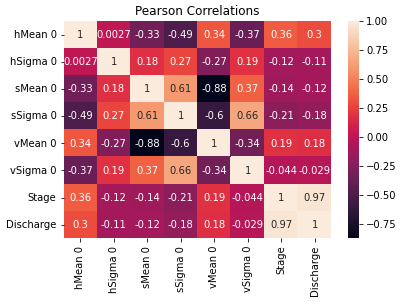
\includegraphics{images/Corr_pearson6.PNG} 
            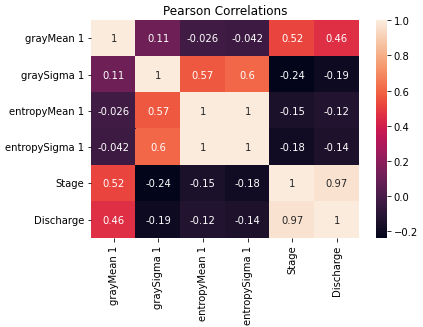
\includegraphics{images/Corr_pearson7.PNG} 
            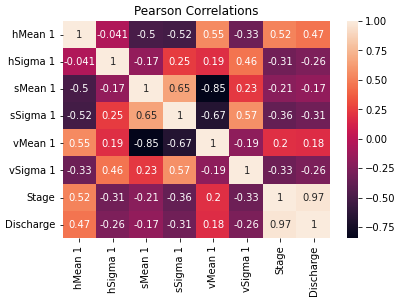
\includegraphics{images/Corr_pearson8.PNG}
            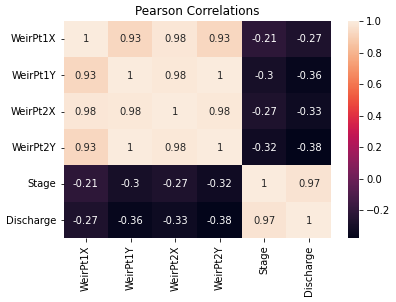
\includegraphics{images/Corr_pearson9.PNG}
            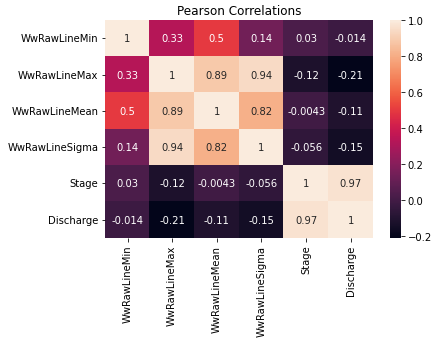
\includegraphics{images/Corr_pearson10.PNG}
       \end{center}   


        Tras analizar los resultados optamos por las siguientes variables:
            \begin{itemize}
                \item sSigma 
                \item grayMean 0 
                \item hMean 0 
                \item grayMean 1 
                \item hMean 1 
                \item sMean 
                \item sSigma 1
                \item WeirPt1Y 
                \item WeirPt2X 
                \item WeirPt2Y 
            \end{itemize}
    
        Podemos observar sus correlaciones en este último gráfico

         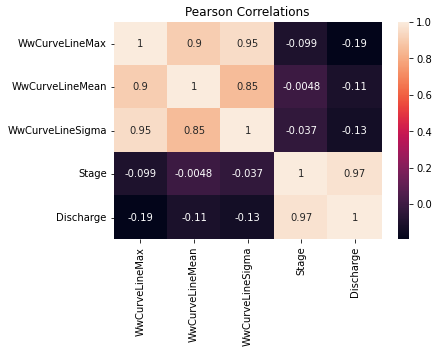
\includegraphics{images/Corr_pearson11.PNG} 



    \section{Desarrollo del modelo con los datos}



\end{document}
